\documentclass[12pt,a4paper]{article}

% ── Geometry & spacing ──────────────────────────────────────
\usepackage[margin=2.5cm]{geometry}
\setlength{\headheight}{14.5pt}
\addtolength{\topmargin}{-2.5pt}
\setlength{\parindent}{1.25em}
\setlength{\parskip}{0pt}

% ── Encoding & language ─────────────────────────────────────
\usepackage[T1]{fontenc}
\usepackage[utf8]{inputenc}
% Swap the two lines below to switch language:
% \usepackage[english]{babel}       
\usepackage[indonesian]{babel}     % Bahasa Indonesia

% ── Font ────────────────────────────────────────────────────
\usepackage{lmodern}

% ── Math ────────────────────────────────────────────────────
\usepackage{amsmath, amssymb, amsthm}
\usepackage{mathtools}

% ── Graphics & figures ──────────────────────────────────────
\usepackage{graphicx}
\usepackage{float}
\usepackage{caption}
\usepackage{subcaption}
\graphicspath{{doc/}}

% ── Tables ──────────────────────────────────────────────────
\usepackage{booktabs}
\usepackage{array}
\usepackage{longtable}

% ── Lists ───────────────────────────────────────────────────
\usepackage{enumitem}

% ── Code listings ───────────────────────────────────────────
\usepackage{listings}
\usepackage{xcolor}

\definecolor{codebg}{RGB}{245,245,245}
\definecolor{codeframe}{RGB}{200,200,200}
\definecolor{codekw}{RGB}{0,0,180}
\definecolor{codecomment}{RGB}{60,128,49}
\definecolor{codestring}{RGB}{163,21,21}

\lstdefinestyle{default}{
  backgroundcolor=\color{codebg},
  basicstyle=\ttfamily\small,
  breaklines=true,
  breakatwhitespace=false,
  tabsize=2,
  showstringspaces=false,
  frame=single,
  rulecolor=\color{codeframe},
  numbers=left,
  numberstyle=\tiny\color{gray},
  numbersep=8pt,
  xleftmargin=2.5em,
  framexleftmargin=2em,
  keywordstyle=\color{codekw}\bfseries,
  commentstyle=\color{codecomment}\itshape,
  stringstyle=\color{codestring},
}
\lstdefinestyle{go}{style=default, language=Python}    % closest builtin
\lstdefinestyle{python}{style=default, language=Python}
\lstdefinestyle{java}{style=default, language=Java}
\lstdefinestyle{cpp}{style=default, language=C++}
\lstdefinestyle{bash}{style=default, language=bash}

\lstset{style=default}   % global default

% ── Boxes (for tips / callouts) ──────────────────────────────
\usepackage{tcolorbox}
\tcbuselibrary{listings, skins, breakable}

\newtcolorbox{infobox}[1][Note]{
  colback=blue!5!white, colframe=blue!50!black,
  fonttitle=\bfseries, title=#1,
  breakable
}
\newtcolorbox{warnbox}[1][Warning]{
  colback=orange!10!white, colframe=orange!80!black,
  fonttitle=\bfseries, title=#1,
  breakable
}

\usepackage{hyperref}
\usepackage{xurl}
\hypersetup{colorlinks=true, linkcolor=black, urlcolor=blue, citecolor=black}

\usepackage{siunitx}

\usepackage{fancyhdr}
\pagestyle{fancy}
\fancyhf{}
\lhead{\CourseCode{} -- \CourseName}
\rhead{\thepage}

% ── First-line indent on all sections ───────────────────────
\usepackage{indentfirst}

\newcommand{\CourseCode}{IF2224}
\newcommand{\CourseName}{Teori Bahasa Formal dan Otomata}
\newcommand{\AssignmentTitle}{Laporan Tugas Besar}
\newcommand{\AssignmentSubtitle}{Milestone 2: Syntax Analysis}
\newcommand{\Semester}{Semester II / 2025--2026}

% Team / group
\newcommand{\GroupName}{GTFOTBFO (HBB)}
\newcommand{\MemberA}{Nathanael Imandatua Manurung - 13524021}
\newcommand{\MemberB}{Nicholas Wise Saragih Sumbayak - 13524037}
\newcommand{\MemberC}{Kurt Mikhael Purba - 13524065}
\newcommand{\MemberD}{Rava Khoman Tuah Saragih - 13524107}


% Institution
\newcommand{\Lab}{Laboratorium Ilmu dan Rekayasa Komputasi}
\newcommand{\Program}{Teknik Informatika}
\newcommand{\Faculty}{Sekolah Teknik Elektro dan Informatika}
\newcommand{\University}{Institut Teknologi Bandung}

% Repository link (used in Appendix)
\newcommand{\RepoURL}{https://github.com/nicholaswisee/HBB-Tubes-IF2224-2026}
\newcommand{\DeployURL}{https://your-deployment-url.example.com}
\newcommand{\DFAURL}{https://drive.google.com/file/d/1XT-esS_K76ImoWZUwJKy43QvJW_NdP0a/view}

\begin{document}

\begin{titlepage}
  \begin{center}
    \vspace*{1cm}
    {\Huge \textbf{\AssignmentTitle}}\\[0.4cm]
    {\Large \textsc{\CourseCode{} \CourseName}}\\[0.2cm]
    {\large \textsc{\AssignmentSubtitle}}\\[0.2cm]
    {\large \textsc{\Semester}}\\[2cm]

    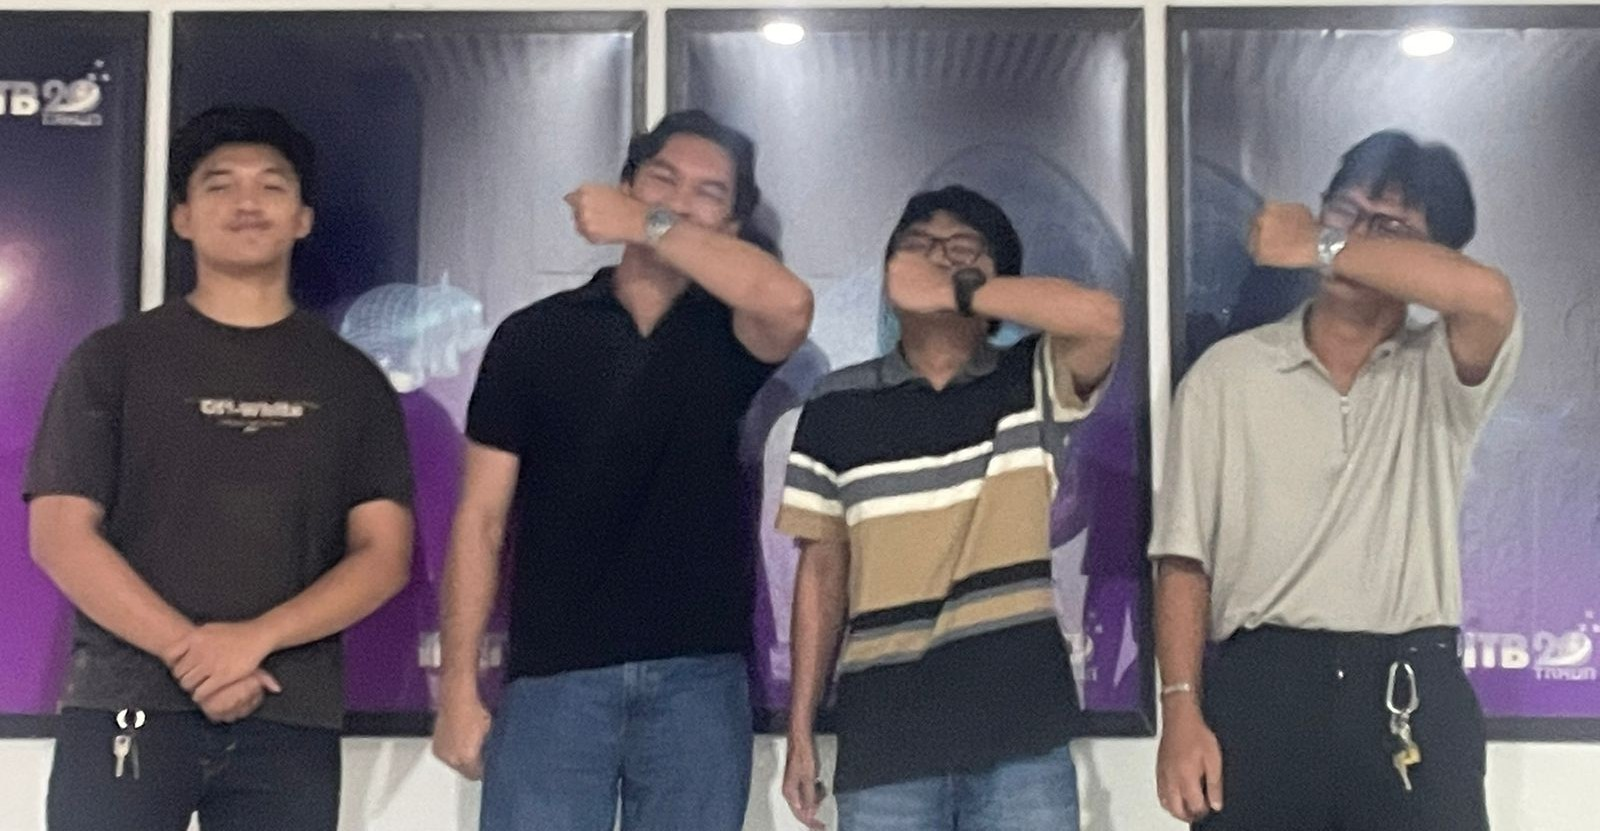
\includegraphics[height=8cm]{nael.jpeg}\\[2cm]

    {\large \textbf{Disusun oleh:}}\\[0.3cm]
    {\large
      \textbf{\GroupName}\\[0.25cm]
      \MemberA\\
      \MemberB\\
      \MemberC\\
      \MemberD\\
    }

    \vfill

    {\large \textsc{\Lab}}\\[0.15cm]
    {\large \textsc{Program Studi \Program}}\\[0.15cm]
    {\large \textsc{\Faculty}}\\[0.15cm]
    {\large \textsc{\University}}\\
  \end{center}
\end{titlepage}

\tableofcontents
\newpage

\section{Pendahuluan}

Pada tahap sebelumnya, telah berhasil dibangun sebuah \textit{lexical analyzer} (lexer) yang mampu membaca kode sumber bahasa Arion dan mengubahnya menjadi daftar token. Setiap token merepresentasikan unit leksikal terkecil dari program, seperti kata kunci, identifier, konstanta, dan operator. Meskipun lexer telah berfungsi dengan baik dalam mengenali dan mengklasifikasikan token-token tersebut, lexer belum mampu memastikan apakah urutan token tersebut membentuk struktur program yang valid sesuai dengan aturan tata bahasa (\textit{grammar}) bahasa Arion.

Proses transformasi kode sumber menjadi program yang dapat dijalankan melibatkan beberapa tahap berurutan. Setelah analisis leksikal selesai, tahap berikutnya adalah analisis sintaktik (\textit{syntax analysis}) atau yang sering disebut \textit{parsing}. Pada tahap ini, parser menerima daftar token dari lexer dan memeriksa apakah urutan token tersebut sesuai dengan aturan grammar yang didefinisikan untuk bahasa Arion. Parser kemudian membangun sebuah struktur hierarkis yang disebut Parse Tree, yang merepresentasikan hubungan struktural antar-komponen program secara menyeluruh.

\begin{figure}[H]
\centering
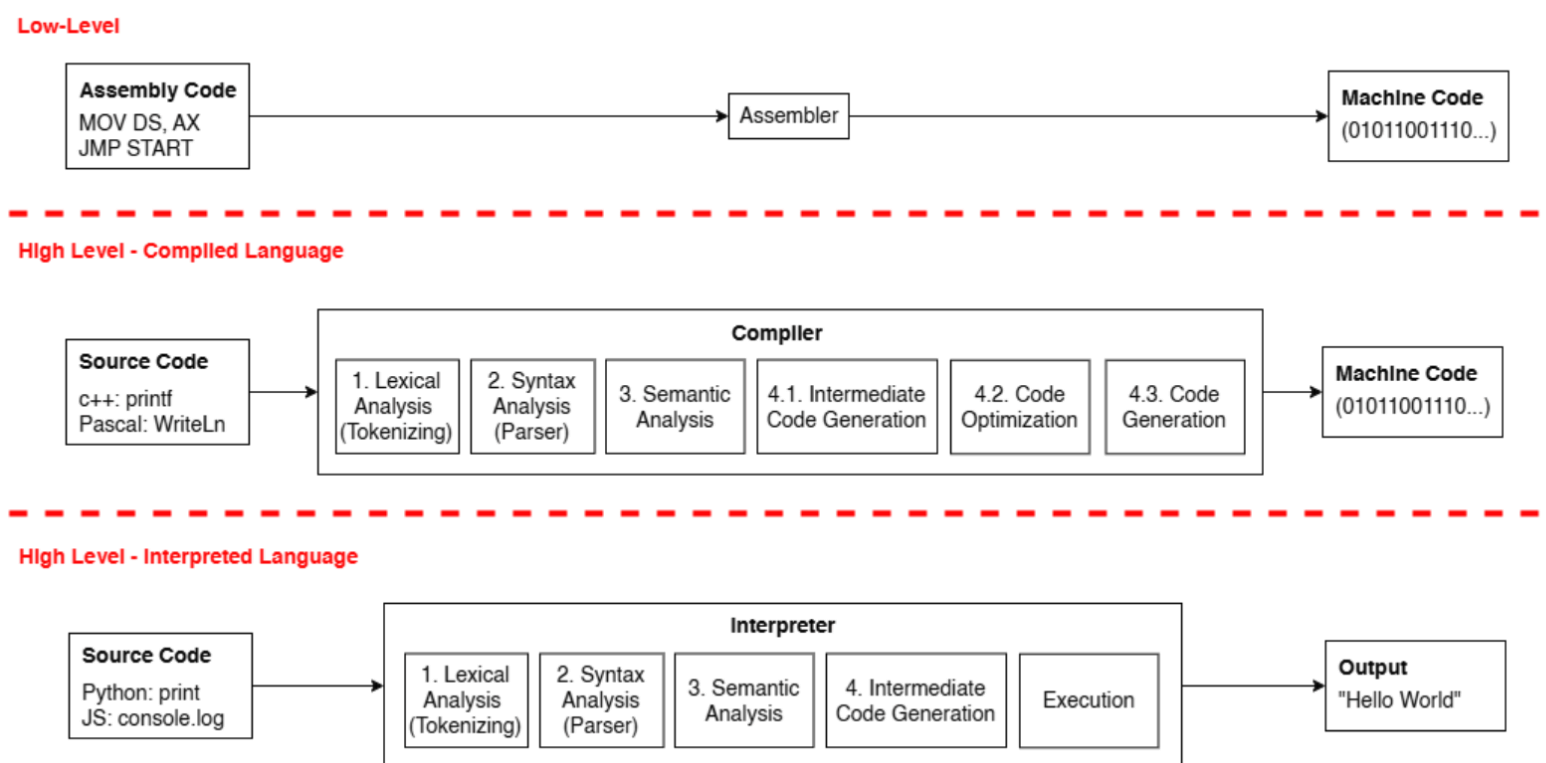
\includegraphics[width=0.8\textwidth]{tipe-bahasa.png}
\caption{Tahap-tahap kompilasi dalam compiler}
\caption*{Sumber: Asisten IF2224}
\end{figure}

Parse Tree adalah representasi lengkap dari struktur sintaks program sesuai dengan grammar bahasa yang digunakan. Setiap node dalam parse tree merepresentasikan simbol non-terminal atau terminal dari aturan produksi grammar. Berbeda dengan Abstract Syntax Tree (AST) yang menyederhanakan struktur dengan menghapus node-node informatif, Parse Tree memuat semua detail simbol seolah-olah seseorang menggambarkan semua langkah produksi secara lengkap. Parse Tree berguna untuk menunjukkan bagaimana token-token hasil lexical analysis membentuk struktur program yang sesuai dengan aturan grammar.

\subsection{Latar Belakang}
Proses kompilasi suatu bahasa pemrograman terdiri atas beberapa tahap yang
saling berkaitan, dimulai dari analisis leksikal (\textit{lexical analysis}),
analisis sintaktik, analisis semantik, hingga pembangkitan kode (\textit{code
generation}). Setelah lexer berhasil mengonversi kode sumber menjadi deretan
token, tahap analisis sintaktik menjadi penting untuk memverifikasi apakah
urutan token tersebut memenuhi aturan tata bahasa yang telah didefinisikan.

Pada tugas besar mata kuliah IF2224 Teori Bahasa Formal dan Otomata, mahasiswa diminta untuk membangun sebuah \textit{compiler} sederhana untuk bahasa pemrograman Arion, yaitu bahasa bertipe Pascal. Milestone kedua ini berfokus pada pembangunan \textit{syntax analyzer} (parser) yang mampu memeriksa urutan token dari lexer dan membangun Parse Tree sesuai dengan aturan grammar bahasa Arion. Parser yang dibangun menggunakan algoritma \textit{Recursive Descent} yang mengimplementasikan setiap aturan produksi dalam grammar sebagai fungsi-fungsi rekursif.

\subsection{Rumusan Masalah}
Bagaimana merancang dan mengimplementasikan sebuah \textit{syntax analyzer} berbasis \textit{Recursive Descent Parser} yang mampu:
\begin{enumerate}[label=\arabic*.]
  \item Membaca daftar token dari keluaran \textit{lexical analyzer}.
  \item Memeriksa apakah urutan token sesuai dengan aturan tata bahasa (\textit{grammar}) bahasa Arion.
  \item Mendeteksi dan melaporkan kesalahan sintaks (\textit{syntax error}) dengan informasi lokasi yang akurat.
  \item Membangun Parse Tree yang merepresentasikan struktur hierarkis program sumber.
\end{enumerate}

\subsection{Gambaran Umum Sistem}
Sistem yang dibangun merupakan sebuah \textit{syntax analyzer} untuk bahasa Arion yang diimplementasikan dalam bahasa C++20. Parser ini menerima daftar token dari lexer (berupa berkas teks yang berisi token-token), memproses setiap token menggunakan algoritma Recursive Descent, dan menghasilkan Parse Tree sebagai keluaran. Sistem terdiri atas beberapa komponen utama: Parser (mesin Recursive Descent), Node (struktur data node pada Parse Tree), TreeBuilder (konstruktor Parse Tree), dan ErrorHandler (pelaporan kesalahan sintaks).

\subsection{Spesifikasi Umum}
\begin{enumerate}[label=\arabic*.]
  \item Menggunakan algoritma \textit{Recursive Descent} dengan grammar yang
      dispesifikasikan dalam program.
  \item Mendukung seluruh node Parse Tree sesuai spesifikasi: program, program-header, declaration-part, compound-statement, statement, expression, dan lainnya.
  \item Melaporkan kesalahan sintaks dengan pesan yang informatif dan akurat.
  \item Menghasilkan Parse Tree yang terformat dengan jelas, ditampilkan ke terminal dan disimpan ke dalam berkas teks.
  \item Menerima masukan berupa berkas daftar token hasil dari lexer milestone pertama.
\end{enumerate}


\section{Dasar Teori}

\subsection{Pendefinisian Bahasa Pemrograman}
Bahasa Pemrograman adalah cara manusia untuk dapat memberikan perintah
(\textit{instruction}) kepada sebuah komputer. Setiap bahasa pemrograman
memiliki kata kunci dan aturannya masing-masing serta makna dari kata-kata itu
yang disebut sintaks(\textit{syntax}) dan semantik (\textit{semantics}).
Input yang terdapat kesalahan pada tingkat sintaks berarti input tersebut tidak
valid untuk bahasa pemrograman tersebut, sedangkan kesalahan pada tingkat
semantik umumnya berbentuk kesalahan logika.

\subsubsection{Hierarki Bahasa Pemrograman}
Berdasarkan tingkat abstraksinya, bahasa pemrograman diklasifikasikan menjadi dua kategori utama:
\begin{itemize}
\item \textbf{\textit{Low-Level Language} (Bahasa Tingkat Rendah)}: Bahasa yang instruksinya mendekati arsitektur perangkat keras dan bahasa mesin (biner 0 dan 1). Contohnya adalah \textit{Assembly}, yang memerlukan \textit{Assembler} untuk menerjemahkan kode menjadi instruksi yang dapat dipahami CPU.
\item \textbf{\textit{High-Level Language} (Bahasa Tingkat Tinggi)}: Bahasa yang dirancang agar lebih mudah dibaca dan dipahami oleh manusia karena menggunakan kosakata yang menyerupai bahasa natural. Semakin tinggi tingkat bahasa tersebut, semakin banyak tahapan pemrosesan yang diperlukan untuk mengubahnya menjadi kode mesin. Contoh bahasa tingkat tinggi antara lain Pascal, C++, Python, dan Java.
\end{itemize}

\subsubsection{\textit{Compiler} dan \textit{Interpreter} }
Untuk menjalankan kode sumber yang ditulis dalam bahasa tingkat tinggi,
diperlukan sebuah perangkat lunak penerjemah yang mengubah kode tersebut menjadi
format yang dapat dieksekusi oleh mesin. Secara umum, terdapat dua mekanisme
utama untuk mengubah bahasa tingkat tinggi ke bahasa mesin:

\begin{enumerate}
\item \textbf{\textit{Compiler} (Kompilator)}:
\textit{Compiler} adalah program yang menerjemahkan seluruh \textit{source code}
secara utuh menjadi kode mesin (biasanya dalam bentuk \textit{Object File})
sebelum program dijalankan. Proses kompilasi pada \textit{compiler} umumnya
terdiri dari empat tahapan utama: \textit{Lexical Analysis}, \textit{Syntax
Analysis}, \textit{Semantic Analysis}, dan \textit{Intermediate Code
Generation}. Karakteristik utama \textit{compiler} adalah jika terdeteksi adanya
kesalahan (\textit{error}) di dalam \textit{source code}, maka seluruh proses
kompilasi akan gagal dan program tidak dapat dijalankan.

\item \textbf{\textit{Interpreter}}: 
Berbeda dengan \textit{compiler}, \textit{interpreter} memproses kode sumber
baris demi baris secara langsung. \textit{Interpreter} membaca,
menerjemahkan, dan langsung mengeksekusi kode mesin tersebut baris demi baris.
Hal ini memungkinkan program tetap berjalan normal hingga baris sebelum
ditemukannya kesalahan; misalnya, jika terdapat \textit{error} pada baris ke-10,
baris 1 sampai 9 akan tetap berhasil dieksekusi. Meskipun mekanisme eksekusinya
berbeda, \textit{interpreter} sebenarnya memiliki tahapan pemrosesan internal
yang serupa dengan \textit{compiler}.

\end{enumerate}

\subsection{Teori Kompilator (\textit{Compiler Theory})}

Proses kompilasi adalah urutan dari berbagai fase (\textit{phases}) yang bekerja secara berurutan. Setiap fase mengambil input dari tahap sebelumnya, memprosesnya, dan memberikan output yang akan digunakan sebagai input untuk fase berikutnya. Secara umum, arsitektur sebuah kompilator terdiri dari fase-fase berikut:

\begin{enumerate}
    \item \textbf{\textit{Lexical Analysis}}: Fase pertama yang bekerja sebagai
        pemindai teks (\textit{text scanner}) pada kode sumber. Penjelasan lebih detail mengenai fase ini dibahas pada sub-bab tersendiri di bawah.
    \item \textbf{\textit{Syntax Analysis} (\textit{Parsing})}: Mengambil
        \textit{token} yang dihasilkan oleh \textit{lexical analysis} dan
        membangun pohon sintaksis (\textit{parse tree}). Fase ini memeriksa
        kebenaran susunan \textit{token} berdasarkan aturan tata bahasa
        (\textit{grammar}) kode sumber.
    \item \textbf{\textit{Semantic Analysis}}: Memeriksa apakah pohon sintaksis
        yang dibangun mengikuti aturan semantik bahasa, seperti kecocokan
        operasi tipe data dan memastikan \textit{identifier} telah
        dideklarasikan sebelum digunakan. Fase ini menghasilkan keluaran berupa
        pohon sintaksis yang dianotasi.
    \item \textbf{\textit{Intermediate Code Generation}}: Menghasilkan
        representasi kode perantara untuk mesin abstrak, yang posisinya
        menjembatani antara bahasa tingkat tinggi dan bahasa mesin.
    \item \textbf{\textit{Code Optimization}}: Mengoptimalkan kode perantara
        dengan menghapus baris kode yang tidak perlu dan mengatur ulang urutan
        instruksi. Tujuannya adalah untuk mempercepat eksekusi program tanpa
        membuang sumber daya (\textit{CPU}, memori).
    \item \textbf{\textit{Target Code Generation}}: Merupakan fase sintesis
    akhir (\textit{back-end}) yang menggunakan representasi kode perantara dan
    tabel simbol untuk menghasilkan program target atau bahasa mesin.
\end{enumerate}

\subsubsection{Analisis Sintaksis (\textit{Syntax Analysis})}
Sebagai fokus utama pada \textit{milestone} ini, Analisis Sintaksis atau
\textit{parser} adalah tahapan atau fase kedua dari sebuah kompilator. Fase ini
bertugas untuk memeriksa urutan \textit{token} yang dihasilkan oleh
\textit{lexical analyzer} agar sesuai dengan aturan tata bahasa
(\textit{grammar}) dari bahasa pemrograman yang dikompilasi.  Dalam
mendefinisikan dan melakukan evaluasi aturan sintaks, \textit{parser} secara
umum mengadopsi format tata bahasa bebas konteks atau \textit{Context-Free
Grammar} (CFG).

Berdasarkan prinsip desain kompilator, mekanisme kerja dan tahapan \textit{parser} bertujuan untuk:
\begin{itemize}
    \item \textbf{Memvalidasi Struktur Sintaks}: Memastikan urutan
        \textit{token} membentuk struktur sintaks yang valid.
    \item \textbf{Penanganan Kesalahan Sintaks (\textit{Syntax Error})}:
        Mendeteksi dan melaporkan kesalahan sintaks (\textit{syntax error})
        apabila ditemukan ketidaksesuaiaan.
    \item \textbf{Membangun Representasi Program}: Mempersiapkan representasi
        program untuk tahap kompilasi berikutnya. \textit{Parser} akan membangun
        struktur sintaks hierarkis seperti \textit{Parse Tree} atau
        \textit{Abstract Syntax Tree} (AST).
\end{itemize}


\textit{Parse Tree} adalah representasi lengkap dari struktur sintaks program sesuai dengan \textit{grammar} bahasa yang digunakan. Karena merepresentasikan hierarki secara utuh, setiap \textit{node} di dalam pohon ini memuat semua simbol terminal dan non-terminal. \textit{Parse tree} berguna untuk menunjukkan bagaimana \textit{token-token} hasil \textit{lexical analysis} membentuk struktur program yang sesuai dengan aturan \textit{grammar}.

Secara garis besar, pendekatan \textit{syntax analyzer} dapat diklasifikasikan ke dalam dua jenis \textit{parsing}:
\begin{itemize}
    \item \textbf{\textit{Top-Down Parsing}}: Pendekatan konstruksi \textit{parse tree} yang dimulai dari simpul akar (\textit{root}) dan diturunkan ke arah simpul daun (\textit{leaves}). Implementasi yang umum digunakan pada pendekatan ini adalah algoritma \textit{Recursive Descent}.
    \item \textbf{\textit{Bottom-Up Parsing}}: Pendekatan konstruksi \textit{parse tree} yang dimulai dari simpul daun (\textit{leaves}) dan dikompresi perlahan menuju simpul akar (\textit{root}). Contoh algoritma dari kategori ini adalah \textit{LR Parser}.
\end{itemize}
\subsection{Teori Bahasa Formal dan Otomata}

Berbeda dengan tahap analisis leksikal yang menggunakan \textit{Regular
Expression} dan \textit{Finite Automata} untuk mengenali pola token, tahap
analisis sintaktik menggunakan konsep (\textit{Context-Free Grammar}) sebagai
dasar untuk memeriksa dan membangun struktur program.

\subsubsection{Context-Free Grammar (CFG)}

\textit{Context-Free Grammar} (CFG) adalah formalisme matematis yang digunakan
untuk mendefinisikan sintaks dari bahasa pemrograman. CFG terdiri dari himpunan
simbol terminal, himpunan simbol non-terminal, himpunan aturan produksi, dan
simbol awal. Aturan produksi menentukan bagaimana simbol non-terminal dapat
diturunkan menjadi rangkaian simbol terminal dan non-terminal lainnya.

Secara formal, sebuah CFG didefinisikan sebagai \textit{4-tuple} $(V, T, P, S)$,
yang terdiri dari:
\begin{itemize}
    \item $V$ : Himpunan hingga simbol non-terminal (variabel).
    \item $T$ : Himpunan hingga simbol terminal (token dari lexer).
    \item $P$ : Himpunan aturan produksi yang mendefinisikan bagaimana simbol
        diturunkan.
    \item $S$ : Simbol awal (\textit{start symbol}), di mana $S \in V$.
\end{itemize}

Dalam konteks compiler, simbol terminal berasal dari hasil analisis leksikal (token), sedangkan simbol non-terminal merepresentasikan struktur sintaks program seperti \texttt{<program>}, \texttt{<statement>}, \texttt{<expression>}, dan lainnya.

Sebagai contoh, grammar sederhana untuk ekspresi aritmatika dapat didefinisikan sebagai:
\begin{align*}
E &\rightarrow E + T \mid T \\
T &\rightarrow T \times F \mid F \\
F &\rightarrow (E) \mid \texttt{intcon}
\end{align*}

Aturan produksi ini menunjukkan bahwa sebuah ekspresi $E$ dapat berupa $E + T$ atau simplemente $T$, dan seterusnya.

\subsubsection{Derivasi dan Parse Tree}

Proses penerapan aturan produksi untuk mengubah simbol awal menjadi deretan simbol terminal disebut \textit{derivasi}. Terdapat dua strategi derivasi utama:
\begin{itemize}
    \item \textbf{\textit{Leftmost Derivation}}: Simbol non-terminal paling kiri dikembangkan terlebih dahulu pada setiap langkah.
    \item \textbf{\textit{Rightmost Derivation}}: Simbol non-terminal paling kanan dikembangkan terlebih dahulu pada setiap langkah.
\end{itemize}

Parse Tree adalah representasi visual dari proses derivasi. Setiap node dalam
parse tree merepresentasikan simbol (terminal atau non-terminal), dan setiap
edge merepresentasikan penerapan aturan produksi. Parse Tree memuat seluruh
simbol yang muncul selama derivasi, berbeda dengan Abstract Syntax Tree (AST)
yang menghilangkan node-node informatif.

\subsubsection{Recursive Descent Parser}

\textit{Recursive Descent} adalah algoritma \textit{top-down parsing} yang
mengimplementasikan setiap aturan produksi dalam grammar sebagai fungsi
rekursif. Setiap fungsi bertanggung jawab untuk mengenali simbol non-terminal
tertentu dan semua turunannya.

Prinsip kerja Recursive Descent adalah:
\begin{enumerate}
    \item Setiap simbol non-terminal diimplementasikan sebagai satu fungsi.
    \item Fungsi membaca token dari input dan memeriksa apakah token tersebut
        sesuai dengan ekspektasi berdasarkan aturan produksi.
    \item Jika ditemukan simbol non-terminal di ruas kanan produksi, fungsi
        memanggil fungsi lain yang berhubungan dengannya.
    \item Jika token yang dibaca tidak sesuai, parser melaporkan kesalahan sintaks.
\end{enumerate}

Keunggulan Recursive Descent adalah kesederhanaan implementasinya dan kemudahan dalam memahami alur parsing. Namun, kelemahannya adalah ketidakmampuan untuk menangani \textit{left recursion} (produk seperti $A \rightarrow A \alpha$) yang dapat menyebabkan infinite recursion.

\section{Perancangan Syntax Analyzer}

Perancangan \textit{syntax analyzer} untuk bahasa Arion didasarkan pada aturan tata bahasa bebas konteks (\textit{Context-Free Grammar}) yang mendefinisikan struktur sintaks bahasa secara hierarkis. Parser yang dibangun menggunakan algoritma \textit{Recursive Descent} dengan pendekatan \textit{top-down parsing}. Pada bagian ini, dijelaskan rancangan grammar bahasa Arion, perancangan Parse Tree, algoritma Recursive Descent, strategi penanganan kesalahan, dan alur kerja program.

\subsection{Grammar Bahasa Arion}

Grammar bahasa Arion didefinisikan dalam bentuk aturan produksi (\textit{production rules}) yang terdiri atas simbol non-terminal (struktur sintaks) dan simbol terminal (token hasil lexer). Simbol awal (\textit{start symbol}) dari grammar ini adalah \texttt{<program>}. Berikut adalah seluruh aturan produksi yang digunakan dalam perancangan parser.

\subsubsection{Struktur Program}
\begin{align*}
\langle \text{program} \rangle &\rightarrow \langle \text{program-header} \rangle \; \langle \text{declaration-part} \rangle \; \langle \text{compound-statement} \rangle \; \texttt{period} \\
\langle \text{program-header} \rangle &\rightarrow \texttt{programsy} \; \texttt{ident} \; \texttt{semicolon} \\
\langle \text{block} \rangle &\rightarrow \langle \text{declaration-part} \rangle \; \langle \text{compound-statement} \rangle
\end{align*}

\subsubsection{Deklarasi}
\begin{align*}
\langle \text{declaration-part} \rangle &\rightarrow ( \langle \text{const-declaration} \rangle )^* \; ( \langle \text{type-declaration} \rangle )^* \\
&\quad\; ( \langle \text{var-declaration} \rangle )^* \; ( \langle \text{subprogram-declaration} \rangle )^* \\
\langle \text{const-declaration} \rangle &\rightarrow \texttt{constsy} \; ( \texttt{ident} \; \texttt{eql} \; \langle \text{constant} \rangle \; \texttt{semicolon} )^+ \\
\langle \text{constant} \rangle &\rightarrow \texttt{charcon} \;|\; \texttt{string} \;|\; [ \texttt{plus} \;|\; \texttt{minus} ] \; ( \texttt{ident} \;|\; \texttt{intcon} \;|\; \texttt{realcon} ) \\
\langle \text{type-declaration} \rangle &\rightarrow \texttt{typesy} \; ( \texttt{ident} \; \texttt{eql} \; \langle \text{type} \rangle \; \texttt{semicolon} )^+ \\
\langle \text{type} \rangle &\rightarrow \texttt{ident} \;|\; \langle \text{array-type} \rangle \;|\; \langle \text{range} \rangle \;|\; \langle \text{enumerated} \rangle \;|\; \langle \text{record-type} \rangle \\
\langle \text{array-type} \rangle &\rightarrow \texttt{arraysy} \; \texttt{lbrack} \; ( \langle \text{range} \rangle \;|\; \texttt{ident} ) \; \texttt{rbrack} \; \texttt{ofsy} \; \langle \text{type} \rangle \\
\langle \text{range} \rangle &\rightarrow \langle \text{expression} \rangle \; \texttt{period} \; \texttt{period} \; \langle \text{expression} \rangle \\
\langle \text{enumerated} \rangle &\rightarrow \texttt{lparent} \; \texttt{ident} \; ( \texttt{comma} \; \texttt{ident} )^* \; \texttt{rparent} \\
\langle \text{record-type} \rangle &\rightarrow \texttt{recordsy} \; \langle \text{field-list} \rangle \; \texttt{endsy} \\
\langle \text{field-list} \rangle &\rightarrow \langle \text{field-part} \rangle \; ( \texttt{semicolon} \; \langle \text{field-part} \rangle )^* \\
\langle \text{field-part} \rangle &\rightarrow \langle \text{identifier-list} \rangle \; \texttt{colon} \; \langle \text{type} \rangle \\
\langle \text{var-declaration} \rangle &\rightarrow \texttt{varsy} \; ( \langle \text{identifier-list} \rangle \; \texttt{colon} \; \langle \text{type} \rangle \; \texttt{semicolon} )^+ \\
\langle \text{identifier-list} \rangle &\rightarrow \texttt{ident} \; ( \texttt{comma} \; \texttt{ident} )^*
\end{align*}

\subsubsection{Subprogram}
\begin{align*}
\langle \text{subprogram-declaration} \rangle &\rightarrow \langle \text{procedure-declaration} \rangle \;|\; \langle \text{function-declaration} \rangle \\
\langle \text{procedure-declaration} \rangle &\rightarrow \texttt{proceduresy} \; \texttt{ident} \; [ \langle \text{formal-parameter-list} \rangle ] \; \texttt{semicolon} \\
&\quad\; \langle \text{block} \rangle \; \texttt{semicolon} \\
\langle \text{function-declaration} \rangle &\rightarrow \texttt{functionsy} \; \texttt{ident} \; [ \langle \text{formal-parameter-list} \rangle ] \; \texttt{colon} \; \texttt{ident} \\
&\quad\; \texttt{semicolon} \; \langle \text{block} \rangle \; \texttt{semicolon} \\
\langle \text{formal-parameter-list} \rangle &\rightarrow \texttt{lparent} \; \langle \text{parameter-group} \rangle \; ( \texttt{semicolon} \; \langle \text{parameter-group} \rangle )^* \; \texttt{rparent} \\
\langle \text{parameter-group} \rangle &\rightarrow \langle \text{identifier-list} \rangle \; \texttt{colon} \; ( \texttt{ident} \;|\; \langle \text{array-type} \rangle )
\end{align*}

\subsubsection{Statement}
\begin{align*}
\langle \text{compound-statement} \rangle &\rightarrow \texttt{beginsy} \; \langle \text{statement-list} \rangle \; \texttt{endsy} \\
\langle \text{statement-list} \rangle &\rightarrow \langle \text{statement} \rangle \; ( \texttt{semicolon} \; \langle \text{statement} \rangle )^* \\
\langle \text{statement} \rangle &\rightarrow \langle \text{assignment-statement} \rangle \;|\; \langle \text{if-statement} \rangle \;|\; \langle \text{case-statement} \rangle \\
&\quad\;|\; \langle \text{while-statement} \rangle \;|\; \langle \text{repeat-statement} \rangle \;|\; \langle \text{for-statement} \rangle \\
&\quad\;|\; \langle \text{procedure/function-call} \rangle \;|\; \epsilon \\
\langle \text{assignment-statement} \rangle &\rightarrow \langle \text{variable} \rangle \; \texttt{becomes} \; \langle \text{expression} \rangle \\
\langle \text{if-statement} \rangle &\rightarrow \texttt{ifsy} \; \langle \text{expression} \rangle \; \texttt{thensy} \; \langle \text{statement} \rangle \\
&\quad\;[ \texttt{elsesy} \; \langle \text{statement} \rangle ] \\
\langle \text{case-statement} \rangle &\rightarrow \texttt{casesy} \; \langle \text{expression} \rangle \; \texttt{ofsy} \; \langle \text{case-block} \rangle \; \texttt{endsy} \\
\langle \text{case-block} \rangle &\rightarrow \langle \text{constant} \rangle \; ( \texttt{comma} \; \langle \text{constant} \rangle )^* \; \texttt{colon} \; \langle \text{statement} \rangle \\
&\quad\; ( \texttt{semicolon} \; \langle \text{case-block} \rangle )^* \\
\langle \text{while-statement} \rangle &\rightarrow \texttt{whilesy} \; \langle \text{expression} \rangle \; \texttt{dosy} \; \langle \text{statement} \rangle \\
\langle \text{repeat-statement} \rangle &\rightarrow \texttt{repeatsy} \; \langle \text{statement-list} \rangle \; \texttt{untilsy} \; \langle \text{expression} \rangle \\
\langle \text{for-statement} \rangle &\rightarrow \texttt{forsy} \; \texttt{ident} \; \texttt{becomes} \; \langle \text{expression} \rangle \\
&\quad\; ( \texttt{tosy} \;|\; \texttt{downtosy} ) \; \langle \text{expression} \rangle \; \texttt{dosy} \; \langle \text{statement} \rangle \\
\langle \text{procedure/function-call} \rangle &\rightarrow \texttt{ident} \; [ \texttt{lparent} \; \langle \text{parameter-list} \rangle \; \texttt{rparent} ] \\
\langle \text{parameter-list} \rangle &\rightarrow \langle \text{expression} \rangle \; ( \texttt{comma} \; \langle \text{expression} \rangle )^*
\end{align*}

\subsubsection{Ekspresi}
\begin{align*}
\langle \text{expression} \rangle &\rightarrow \langle \text{simple-expression} \rangle \\
&\quad\;[ \langle \text{relational-operator} \rangle \; \langle \text{simple-expression} \rangle ] \\
\langle \text{simple-expression} \rangle &\rightarrow [ \texttt{plus} \;|\; \texttt{minus} ] \; \langle \text{term} \rangle \\
&\quad\; ( \texttt{plus} \;|\; \texttt{minus} \;|\; \texttt{orsy} ) \; \langle \text{term} \rangle )^* \\
\langle \text{term} \rangle &\rightarrow \langle \text{factor} \rangle \; ( ( \texttt{times} \;|\; \texttt{rdiv} \;|\; \texttt{idiv} \;|\; \texttt{imod} \;|\; \texttt{andsy} ) \; \langle \text{factor} \rangle )^* \\
\langle \text{factor} \rangle &\rightarrow \texttt{intcon} \;|\; \texttt{realcon} \;|\; \texttt{charcon} \;|\; \texttt{string} \;|\; \langle \text{variable} \rangle \\
&\quad\;|\; \langle \text{procedure/function-call} \rangle \;|\; ( \langle \text{expression} \rangle ) \;|\; \texttt{notsy} \; \langle \text{factor} \rangle
\end{align*}

\subsubsection{Variable}
\begin{align*}
\langle \text{variable} \rangle &\rightarrow \texttt{ident} \; ( \langle \text{component-variable} \rangle )^* \\
\langle \text{component-variable} \rangle &\rightarrow \texttt{lbrack} \; \langle \text{index-list} \rangle \; \texttt{rbrack} \;|\; \texttt{period} \; \texttt{ident} \\
\langle \text{index-list} \rangle &\rightarrow ( \texttt{intcon} \;|\; \texttt{charcon} \;|\; \texttt{ident} ) \; ( \texttt{comma} \; ( \texttt{intcon} \;|\; \texttt{charcon} \;|\; \texttt{ident} ) )^*
\end{align*}

\subsection{Perancangan Parse Tree}

Parse Tree yang dihasilkan oleh parser merupakan representasi hierarkis dari
struktur sintaks program. Setiap simpul (\textit{node}) dalam Parse Tree memuat
label yang menunjukkan simbol terminal atau non-terminal yang direpresentasikan.
Simpul non-terminal diberi label dengan nama aturan produksi dalam tanda kurung
sudut (misalnya \texttt{<program>}, \texttt{<expression>}), sedangkan simpul
terminal diberi label sesuai representasi token dari lexer (misalnya
\texttt{programsy}, \texttt{ident(Hello)}, \texttt{semicolon}).

Struktur data yang digunakan untuk merepresentasikan Parse Tree terdiri
dari label string yang mengidentifikasi node (terminal atau non-terminal dan
daftar anak (sub-pohon) yang terurut sesuai urutan dalam aturan
produksi. Setiap node non-terminal dibuat dengan menciptakan node baru, kemudian
menambahkan node-node anak sesuai dengan aturan produksi yang sedang diproses.
Node terminal dibuat dengan membungkus token yang telah dikonsumsi dari aliran
masukan.

\subsection{Perancangan Algoritma Recursive Descent}

Algoritma Recursive Descent dirancang dengan mengimplementasikan setiap aturan produksi dalam grammar sebagai fungsi rekursif. Setiap fungsi:
\begin{enumerate}
    \item Membuat node Parse Tree baru dengan label non-terminal yang sesuai.
    \item Memeriksa token saat ini (\textit{lookahead}) untuk menentukan cabang produksi yang akan diambil.
    \item Mengonsumsi token terminal yang sesuai atau memanggil fungsi non-terminal lain secara rekursif.
    \item Mengembalikan node yang telah terisi lengkap dengan anak-anaknya.
\end{enumerate}

Dalam perancangan ini, terdapat beberapa strategi disambiguasi untuk menangani kasus di mana satu token dapat mengawali beberapa aturan produksi berbeda:
\begin{itemize}
    \item \textbf{Statement vs Assignment vs Function Call}: Ketika parser menemukan token \texttt{ident}, parser menyimpan posisi saat ini, mencoba mem-parsing sebagai \texttt{<variable>}, lalu memeriksa apakah token berikutnya adalah \texttt{becomes} (\texttt{:=}). Jika ya, diinterpretasikan sebagai \texttt{<assignment-statement>}; jika tidak, diinterpretasikan sebagai \texttt{<procedure/function-call>}.
    \item \textbf{Factor: variable vs function call}: Dalam \texttt{<factor>}, saat menemukan \texttt{ident}, parser melihat satu token ke depan (\textit{lookahead}) untuk memeriksa apakah terdapat \texttt{lparent}. Jika ya, diinterpretasikan sebagai pemanggilan fungsi; jika tidak, sebagai variable.
    \item \textbf{Range vs ident dalam type}: Dalam \texttt{<type>}, token \texttt{ident} bisa merupakan tipe sederhana atau awal dari \texttt{<range>}. Parser memeriksa keberadaan dua titik berurutan (\texttt{period period}) setelah ekspresi untuk menentukan interpretasi.
\end{itemize}

\subsection{Strategi Penanganan Kesalahan}

Parser dirancang untuk mendeteksi dan melaporkan kesalahan sintaks dengan informasi yang informatif. Strategi yang digunakan meliputi:
\begin{itemize}
    \item \textbf{Error detection}: Setiap fungsi parsing memeriksa token yang diharapkan. Jika token tidak sesuai dengan yang diharapkan, parser segera melaporkan kesalahan.
    \item \textbf{Pesan error informatif}: Pesan kesalahan mencakup nomor baris, deskripsi kesalahan, dan token yang ditemukan (misalnya \texttt{"Syntax error on line 3: Expected ';' after program name (got period)"}).
    \item \textbf{\textit{Error recovery}}: Parser menggunakan pendekatan \textit{panic mode}, yaitu melompati token hingga menemukan token sinkronisasi (seperti \texttt{semicolon}, \texttt{endsy}, atau \texttt{beginsy}) untuk melanjutkan parsing.
\end{itemize}

\subsection{Alur Program}

Alur kerja program secara keseluruhan adalah sebagai berikut:
\begin{enumerate}
    \item Program membaca berkas kode sumber dari direktori \texttt{test/input/}.
    \item \texttt{Scanner} melakukan analisis leksikal dan menghasilkan daftar token.
    \item Token-token tersebut ditampilkan ke terminal untuk verifikasi.
    \item \texttt{Parser} menerima daftar token dan melakukan analisis sintaks dengan algoritma Recursive Descent untuk membangun Parse Tree.
    \item Parse Tree yang dihasilkan ditampilkan ke terminal dengan format hierarkis dan disimpan ke dalam berkas teks di direktori \texttt{test/output/}.
\end{enumerate}

\section{Implementasi Parser}

Parser pada compiler Arion diimplementasikan menggunakan algoritma Recursive Descent dalam bahasa C++20. Setiap aturan produksi dalam grammar bahasa Arion direpresentasikan sebagai satu fungsi yang mengembalikan node Parse Tree. Implementasi ini terletak pada direktori \texttt{src/syntax/} dengan struktur kelas yang terdefinisi dengan baik.

\subsection{Struktur Kelas Parser}

Kelas \texttt{Parser} didefinisikan dalam berkas \texttt{Parser.hpp} dan diimplementasikan dalam \texttt{Parser.cpp}. Kelas ini menyimpan daftar token sebagai masukan dan sebuah pointer posisi (\texttt{pos}) untuk menelusuri token secara sekuensial.

\begin{lstlisting}[style=cpp, caption={Deklarasi kelas Parser}]
class Parser {
  public:
    explicit Parser(const std::vector<Token> &tokens);
    std::shared_ptr<ParseTreeNode> parse();

  private:
    std::vector<Token> tokens;
    size_t pos = 0;
    // ...
};
\end{lstlisting}

Kelas \texttt{Parser} menyediakan beberapa metode bantu (\textit{helper methods}) untuk navigasi token yang menjadi fondasi bagi seluruh fungsi parsing:

\begin{itemize}
    \item \texttt{peek()}: Mengembalikan token saat ini tanpa mengonsumsinya.
    \item \texttt{advance()}: Mengonsumsi token saat ini dan memajukan posisi.
    \item \texttt{previous()}: Mengembalikan token yang baru saja dikonsumsi.
    \item \texttt{check(type)}: Memeriksa apakah token saat ini bertipe tertentu.
    \item \texttt{match(type)}: Jika token saat ini sesuai, konsumsi dan kembalikan \texttt{true}.
    \item \texttt{expect(type, errMsg)}: Mengonsumsi token dan melaporkan error jika tidak sesuai.
    \item \texttt{consumeTerminal(type, errMsg)}: Seperti \texttt{expect}, tetapi membungkus hasilnya dalam node Parse Tree.
    \item \texttt{isAtEnd()}: Memeriksa apakah seluruh token telah diproses.
\end{itemize}

\begin{lstlisting}[style=cpp, caption={Implementasi metode bantu parser}]
const Token &Parser::peek() const { return tokens[pos]; }

const Token &Parser::advance() {
    if (!isAtEnd()) pos++;
    return previous();
}

bool Parser::match(TokenType type) {
    if (check(type)) { advance(); return true; }
    return false;
}

const Token &Parser::expect(TokenType type, const string &errMsg) {
    if (check(type)) return advance();
    error(errMsg);
}

shared_ptr<ParseTreeNode>
Parser::consumeTerminal(TokenType type, const string &errMsg) {
    const Token &tok = expect(type, errMsg);
    return makeNode(tok.toString());
}
\end{lstlisting}

\subsection{Struktur Data Parse Tree}

Parse Tree direpresentasikan menggunakan struktur \texttt{ParseTreeNode} yang didefinisikan dalam berkas \texttt{ParseTree.hpp}. Setiap node hanya menyimpan label string dan daftar anak (sub-pohon) yang terurut. Tidak ada pembedaan tipe node -- semua node adalah \texttt{ParseTreeNode} dengan label yang menunjukkan simbol terminal atau non-terminal. Node non-terminal diberi label seperti \texttt{<program>}, \texttt{<expression>}, sedangkan node terminal diberi label sesuai representasi token seperti \texttt{programsy}, \texttt{ident(Hello)}.

\begin{lstlisting}[style=cpp, caption={Struktur data ParseTreeNode}]
struct ParseTreeNode {
    std::string label;
    std::vector<std::shared_ptr<ParseTreeNode>> children;

    explicit ParseTreeNode(const std::string &label) : label(label) {}

    void addChild(std::shared_ptr<ParseTreeNode> child) {
        children.push_back(std::move(child));
    }

    void print(std::ostream &os, const std::string &prefix = "",
               bool isLast = true, bool isRoot = true) const;

    void printToConsole() const;
    void saveToFile(const std::string &path) const;
};

inline std::shared_ptr<ParseTreeNode> makeNode(const std::string &label) {
    return std::make_shared<ParseTreeNode>(label);
}
\end{lstlisting}

Fungsi \texttt{makeNode()} digunakan sebagai \textit{factory function} untuk membuat node baru. Setiap node dapat memiliki banyak anak yang ditambahkan melalui metode \texttt{addChild()}. Node terminal dibuat dengan memanggil \texttt{consumeTerminal()} yang membungkus token hasil parsing menjadi node.

\subsection{Implementasi Aturan Grammar}

Setiap aturan produksi dalam grammar bahasa Arion diimplementasikan sebagai satu fungsi yang mengembalikan \texttt{shared\_ptr<ParseTreeNode>}. Pola implementasi setiap fungsi adalah sama: membuat node baru dengan label non-terminal, kemudian memanggil fungsi \texttt{consumeTerminal()} untuk token terminal atau fungsi parsing lain untuk non-terminal.

\subsubsection{Program dan Struktur Dasar}

\begin{lstlisting}[style=cpp, caption={Implementasi aturan <program> dan <program-header>}]
shared_ptr<ParseTreeNode> Parser::parseProgram() {
    auto node = makeNode("<program>");
    node->addChild(parseProgramHeader());
    node->addChild(parseDeclarationPart());
    node->addChild(parseCompoundStatement());
    node->addChild(consumeTerminal(TokenType::period,
                                   "Expected '.' at end of program"));
    return node;
}

shared_ptr<ParseTreeNode> Parser::parseProgramHeader() {
    auto node = makeNode("<program-header>");
    node->addChild(consumeTerminal(TokenType::programsy,
                                   "Expected 'program'"));
    node->addChild(consumeTerminal(TokenType::ident,
                                   "Expected program name (identifier)"));
    node->addChild(consumeTerminal(TokenType::semicolon,
                                   "Expected ';' after program name"));
    return node;
}
\end{lstlisting}

\subsubsection{Implementasi Deklarasi}

Bagian deklarasi menggunakan perulangan \texttt{while} dan \texttt{do-while} untuk menangani aturan produksi dengan pengulangan (\textit{Kleene star}). Berikut adalah implementasi untuk deklarasi konstanta dan variable:

\begin{lstlisting}[style=cpp, caption={Implementasi deklarasi konstanta}]
shared_ptr<ParseTreeNode> Parser::parseConstDeclaration() {
    auto node = makeNode("<const-declaration>");
    node->addChild(consumeTerminal(TokenType::constsy, "Expected 'const'"));

    do {
        node->addChild(consumeTerminal(TokenType::ident,
                                       "Expected identifier in const declaration"));
        node->addChild(consumeTerminal(TokenType::eql,
                                       "Expected '==' in const declaration"));
        node->addChild(parseConstant());
        node->addChild(consumeTerminal(TokenType::semicolon,
                                       "Expected ';' after constant"));
    } while (check(TokenType::ident));

    return node;
}
\end{lstlisting}

\begin{lstlisting}[style=cpp, caption={Implementasi deklarasi variable}]
shared_ptr<ParseTreeNode> Parser::parseVarDeclaration() {
    auto node = makeNode("<var-declaration>");
    node->addChild(consumeTerminal(TokenType::varsy, "Expected 'var'"));

    do {
        node->addChild(parseIdentifierList());
        node->addChild(consumeTerminal(TokenType::colon,
                                       "Expected ':' in var declaration"));
        node->addChild(parseType());
        node->addChild(consumeTerminal(TokenType::semicolon,
                                       "Expected ';' after var declaration"));
    } while (check(TokenType::ident));

    return node;
}
\end{lstlisting}

\subsubsection{Implementasi Statement}

Statement dalam bahasa Arion terdiri dari beberapa jenis. Implementasi fungsi \texttt{parseStatement()} menggunakan \textit{lookahead} dan \textit{backtracking} untuk membedakan antara \texttt{<assignment-statement>} dan \texttt{<procedure/function-call>}, karena keduanya diawali oleh token \texttt{ident}.

\begin{lstlisting}[style=cpp, caption={Implementasi parsing statement}]
shared_ptr<ParseTreeNode> Parser::parseStatement() {
    auto node = makeNode("<statement>");

    if (check(TokenType::ident)) {
        size_t saved = pos;
        parseVariable();
        bool isAssign = check(TokenType::becomes);
        pos = saved; // backtrack

        if (isAssign) {
            node->addChild(parseAssignmentStatement());
        } else {
            node->addChild(parseProcFuncCall());
        }
    } else if (check(TokenType::ifsy)) {
        node->addChild(parseIfStatement());
    } else if (check(TokenType::whilesy)) {
        node->addChild(parseWhileStatement());
    } else if (check(TokenType::forsy)) {
        node->addChild(parseForStatement());
    } else if (check(TokenType::repeatsy)) {
        node->addChild(parseRepeatStatement());
    } else if (check(TokenType::casesy)) {
        node->addChild(parseCaseStatement());
    } else if (check(TokenType::beginsy)) {
        node->addChild(parseCompoundStatement());
    }

    return node;
}
\end{lstlisting}

\subsubsection{Implementasi Ekspresi}

Ekspresi dalam bahasa Arion mengikuti hierarki operator standar dengan tiga tingkatan prioritas: relasional, aditif, dan multiplikatif. Berikut adalah implementasi untuk ekspresi, simple-ekspresi, dan term:

\begin{lstlisting}[style=cpp, caption={Implementasi ekspresi dengan hierarki operator}]
shared_ptr<ParseTreeNode> Parser::parseExpression() {
    auto node = makeNode("<expression>");
    node->addChild(parseSimpleExpression());

    if (check(TokenType::eql) || check(TokenType::neq) ||
        check(TokenType::gtr) || check(TokenType::geq) ||
        check(TokenType::lss) || check(TokenType::leq)) {
        node->addChild(makeNode(advance().toString()));
        node->addChild(parseSimpleExpression());
    }

    return node;
}

shared_ptr<ParseTreeNode> Parser::parseTerm() {
    auto node = makeNode("<term>");
    node->addChild(parseFactor());

    while (check(TokenType::times) || check(TokenType::rdiv) ||
           check(TokenType::idiv) || check(TokenType::imod) ||
           check(TokenType::andsy)) {
        node->addChild(makeNode(advance().toString()));
        node->addChild(parseFactor());
    }

    return node;
}
\end{lstlisting}

\subsection{Mekanisme Disambiguasi}

Terdapat beberapa kasus ambiguitas dalam grammar yang memerlukan \textit{lookahead} dan \textit{backtracking} untuk diselesaikan:

\begin{enumerate}
    \item \textbf{Statement vs Assignment vs Function Call}: Ketika parser menemukan \texttt{ident}, parser menyimpan posisi token, memanggil \texttt{parseVariable()}, dan memeriksa apakah token berikutnya adalah \texttt{becomes}. Jika iya, parser melakukan \textit{backtrack} ke posisi awal dan memanggil \texttt{parseAssignmentStatement()}. Jika tidak, parser melakukan \textit{backtrack} dan memanggil \texttt{parseProcFuncCall()}.
    \item \textbf{Factor: variable vs function call}: Dalam \texttt{parseFactor()}, setelah membaca \texttt{ident}, parser memeriksa apakah token berikutnya adalah \texttt{lparent}. Jika iya, dilakukan pemanggilan fungsi; jika tidak, diperlakukan sebagai variable.
    \item \textbf{Range vs simple type}: Dalam \texttt{parseType()}, token \texttt{ident} bisa merupakan tipe sederhana atau awal dari range. Parser memeriksa apakah setelah ekspresi terdapat dua titik berurutan (\texttt{period period}) untuk menentukan interpretasi.
\end{enumerate}

\begin{lstlisting}[style=cpp, caption={Disambiguasi factor: variable vs function call}]
shared_ptr<ParseTreeNode> Parser::parseFactor() {
    auto node = makeNode("<factor>");

    if (check(TokenType::intcon) || check(TokenType::realcon) ||
        check(TokenType::charcon) || check(TokenType::string)) {
        node->addChild(makeNode(advance().toString()));
    } else if (check(TokenType::ident)) {
        size_t saved = pos;
        advance();
        if (check(TokenType::lparent)) {
            pos = saved;
            node->addChild(parseProcFuncCall());
        } else {
            pos = saved;
            node->addChild(parseVariable());
        }
    } else if (match(TokenType::lparent)) {
        node->addChild(makeNode(previous().toString()));
        node->addChild(parseExpression());
        node->addChild(consumeTerminal(TokenType::rparent,
                                       "Expected ')'"));
    } else if (match(TokenType::notsy)) {
        node->addChild(makeNode(previous().toString()));
        node->addChild(parseFactor());
    } else {
        error("Expected factor (value, identifier, or expression)");
    }

    return node;
}
\end{lstlisting}

\subsection{Penanganan Kesalahan Sintaks}

Kesalahan sintaks ditangani menggunakan struktur \texttt{SyntaxError} yang merupakan turunan dari \texttt{std::runtime\_error}. Struktur ini menyimpan nomor baris dan pesan kesalahan.

\begin{lstlisting}[style=cpp, caption={Struktur SyntaxError dan fungsi error}]
struct SyntaxError : public std::runtime_error {
    int line;
    SyntaxError(int line, const std::string &msg)
        : std::runtime_error(msg), line(line) {}
};

[[noreturn]] void Parser::error(const string &msg) {
    const Token &tok = peek();
    ostringstream oss;
    oss << "Syntax error on line " << tok.line << ": " << msg
        << " (got " << tok.toString() << ")";
    throw SyntaxError(tok.line, oss.str());
}
\end{lstlisting}

Pada \texttt{main.cpp}, eksepsi \texttt{SyntaxError} ditangkap dan pesan kesalahan ditampilkan ke \texttt{stderr}. Program akan mengembalikan kode keluar 1 jika terjadi kesalahan sintaks.

\begin{lstlisting}[style=cpp, caption={Penanganan error di main.cpp}]
try {
    Parser parser(tokens);
    auto tree = parser.parse();
    tree->printToConsole();
    tree->saveToFile(outFile.string());
} catch (const SyntaxError &e) {
    std::cerr << "\n" << e.what() << "\n";
    return 1;
}
\end{lstlisting}

Fungsi \texttt{expect()} dan \texttt{consumeTerminal()} menjadi garda terdepan dalam deteksi error. Ketika token yang diharapkan tidak ditemukan, parser segera menghentikan proses dan melaporkan kesalahan. Pesan error diformat dengan nomor baris dan token yang ditemukan, sehingga memudahkan pengguna dalam menelusuri sumber kesalahan.

\subsection{Pencetakan dan Penyimpanan Parse Tree}

Parse Tree yang dihasilkan dicetak ke terminal menggunakan format hierarkis dengan garis penghubung (\textit{ASCII art}). Setiap level indentasi menggunakan prefix \texttt{|} untuk cabang yang memiliki saudara setelahnya dan spasi untuk cabang terakhir. Node akar dicetak tanpa prefix, sedangkan node anak menggunakan awalan \texttt{+--} untuk anak terakhir dan \texttt{|--} untuk anak lainnya.

Selain dicetak ke terminal, Parse Tree juga disimpan ke dalam berkas teks di direktori \texttt{test/output/} dengan nama yang sama dengan berkas masukan tetapi berekstensi \texttt{.txt}. Hal ini memungkinkan verifikasi hasil parsing secara otomatis maupun manual.

\begin{lstlisting}[style=cpp, caption={Fungsi pencetakan Parse Tree}]
void ParseTreeNode::print(std::ostream &os, const std::string &prefix,
                           bool isLast, bool isRoot) const {
    if (isRoot) {
        os << label << "\n";
    } else {
        os << prefix;
        os << (isLast ? "+-- " : "|-- ");
        os << label << "\n";
    }

    string childPrefix = isRoot ? "" : prefix + (isLast ? "    " : "|   ");

    for (size_t i = 0; i < children.size(); ++i) {
        children[i]->print(os, childPrefix, i == children.size() - 1, false);
    }
}
\end{lstlisting}

\subsection{Struktur Direktori Proyek}

Struktur direktori proyek untuk milestone kedua adalah sebagai berikut:

\begin{lstlisting}[style=bash, caption={Tata letak direktori proyek}]
HBB-Tubes-IF2224-2026/
    src/
        main.cpp                # Titik masuk program
        lexical/                # Lexical analyzer (milestone 1)
            SourceBuffer.hpp/...
            TokenType.hpp
            Token.hpp/...
            Scanner.hpp/...
            Logger.hpp
        syntax/                 # Syntax analyzer (milestone 2)
            Parser.hpp/cpp      # Implementasi Recursive Descent Parser
            ParseTree.hpp       # Struktur data Parse Tree
    test/
        input/                  # Berkas masukan uji
            pos_*.txt           # Kasus uji positif
            neg_*.txt           # Kasus uji negatif (error)
            edge_*.txt          # Kasus uji batas
    doc/                        # Laporan dan dokumentasi
    Makefile                    # Skrip kompilasi
\end{lstlisting}

% ============================================================
%   SECTION 4 — PENGUJIAN
% ============================================================

\section{Pengujian}

Pengujian dilakukan terhadap berbagai kasus masukan untuk memverifikasi kebenaran lexer. Setiap kasus uji dijalankan dengan perintah \texttt{make run FILE=<nama\_berkas>}. Keluaran pada \texttt{stdout} (daftar token) dan \texttt{stderr} (pesan kesalahan) dibandingkan dengan hasil yang diharapkan.

\subsection{Kasus Uji 1: Kata Kunci dalam Berbagai Huruf Besar/Kecil}
\textbf{Berkas:} \texttt{edge\_keywords\_case.txt}

\textbf{Masukan:}
\begin{lstlisting}[style=default]
BEGIN While PROGRAM
End If THEN
REPEAT downto NOT
DIV Mod Or
\end{lstlisting}

\textbf{Keluaran yang diharapkan:} \texttt{beginsy}, \texttt{whilesy}, \texttt{programsy}, \texttt{endsy}, \texttt{ifsy}, \texttt{thensy}, \texttt{repeatsy}, \texttt{downtosy}, \texttt{notsy}, \texttt{idiv}, \texttt{imod}, \texttt{orsy} --- total 12 token kata kunci.

\begin{figure}[H]
  \centering
  
\includegraphics[width=0.7\textwidth]{testcase1.png}
  \caption{Hasil pengujian kasus uji 1}
\end{figure}

\textbf{Analisis:} Seluruh kata kunci dikenali dengan benar meskipun ditulis dengan variasi huruf besar/kecil, membuktikan bahwa mekanisme \texttt{toLower()} bekerja sesuai spesifikasi.

\subsection{Kasus Uji 2: Ambiguitas Bilangan Riil vs Titik}
\textbf{Berkas:} \texttt{edge\_real\_vs\_period.txt}

\textbf{Masukan:}
\begin{lstlisting}[style=default]
end.
3.14
42.
100.0
5 .3
\end{lstlisting}

\textbf{Keluaran yang diharapkan:} \texttt{endsy}, \texttt{period}, \texttt{realcon (3.14)}, \texttt{intcon (42)}, \texttt{period}, \texttt{realcon (100)}, \texttt{intcon (5)}, \texttt{period}, \texttt{intcon (3)} --- total 9 token.

\begin{figure}[H]
  \centering
  
\includegraphics[width=0.7\textwidth]{testcase2.png}
  \caption{Hasil pengujian kasus uji 2}
\end{figure}

\textbf{Analisis:} Scanner membedakan \texttt{realcon} dan \texttt{period} berdasarkan \textit{lookahead}: titik hanya menjadi bagian bilangan riil jika diikuti digit. Kasus \texttt{42.} menghasilkan \texttt{intcon} + \texttt{period} karena tidak ada digit setelah titik.

\subsection{Kasus Uji 3: Charcon vs String}
\textbf{Berkas:} \texttt{edge\_charcon\_vs\_string.txt}

\textbf{Masukan:}
\begin{lstlisting}[style=default]
'a'
'ab'
'hello world'
'x'
''
\end{lstlisting}

\textbf{Keluaran yang diharapkan:} \texttt{charcon (a)}, \texttt{string (ab)}, \texttt{string (hello world)}, \texttt{charcon (x)}, \texttt{string ()} --- total 5 token.

\begin{figure}[H]
  \centering
  
\includegraphics[width=0.7\textwidth]{testcase3.png}
  \caption{Hasil pengujian kasus uji 3}
\end{figure}

\textbf{Analisis:} Literal dengan tepat satu karakter menjadi \texttt{charcon}; selainnya (termasuk literal kosong \texttt{''}) menjadi \texttt{string}. Perilaku ini sesuai dengan logika \texttt{val.length() == 1} pada \texttt{stringLiteral()}.

\subsection{Kasus Uji 4: Komentar Bersarang dan Berkas Hanya Komentar}
\textbf{Berkas:} \texttt{edge\_nested\_comment.txt} dan \texttt{edge\_only\_comments.txt}

\textbf{Masukan (komentar bersarang):}
\begin{lstlisting}[style=default]
{ comment with { nested brace }
x
\end{lstlisting}

\textbf{Keluaran yang diharapkan:} \texttt{ident (x)} --- komentar dikonsumsi seluruhnya, hanya \texttt{x} yang tersisa.

\textbf{Masukan (hanya komentar):} Berkas yang hanya berisi komentar \texttt{\{\}} dan \texttt{(* *)}.

\textbf{Keluaran yang diharapkan:} Tidak ada token yang dicetak.

\begin{figure}[H]
  \centering
  
\includegraphics[width=0.7\textwidth]{testcase4.png}
  \caption{Hasil pengujian kasus uji 4}
\end{figure}

\textbf{Analisis:} Komentar tidak bersarang; kurung kurawal \texttt{\{} di dalam komentar diabaikan. Berkas yang hanya mengandung komentar menghasilkan keluaran kosong, membuktikan bahwa komentar tidak menghasilkan token.

\subsection{Kasus Uji 5: Konstruksi yang Tidak Ditutup}
\textbf{Berkas:} \texttt{edge\_unterminated.txt} dan \texttt{edge\_unterminated\_comment.txt}

\textbf{Masukan:} String literal tanpa kutip penutup (\texttt{'hello}) dan komentar tanpa kurung penutup (\texttt{\{ never ends}).

\textbf{Keluaran yang diharapkan (stderr):}
\begin{lstlisting}[style=default]
[line 2] Error: Unterminated string or character literal.
[line 2] Error: Unterminated comment.
\end{lstlisting}

\begin{figure}[H]
  \centering
  
\includegraphics[width=0.7\textwidth]{testcase5.png}
  \caption{Hasil pengujian kasus uji 5}
\end{figure}

\textbf{Analisis:} Lexer melaporkan kesalahan dengan nomor baris yang akurat dan tidak mengalami \textit{crash}. Scanner meneruskan pemrosesan setelah menemukan kesalahan (\textit{error recovery}).

\subsection{Kasus Uji 6: Operator \texttt{==} vs Karakter \texttt{=} Tunggal}
\textbf{Berkas:} \texttt{edge\_eql\_vs\_single\_eq.txt}

\textbf{Masukan:}
\begin{lstlisting}[style=default]
x == 5
y = 3
== ==
\end{lstlisting}

\textbf{Keluaran yang diharapkan (stdout):} \texttt{ident (x)}, \texttt{eql}, \texttt{intcon (5)}, \texttt{ident (y)}, \texttt{intcon (3)}, \texttt{eql}, \texttt{eql}.

\textbf{Keluaran yang diharapkan (stderr):} \texttt{[line 2] Error: Unexpected character: =}

\begin{figure}[H]
  \centering
  
\includegraphics[width=0.7\textwidth]{testcase6.png}
  \caption{Hasil pengujian kasus uji 6}
\end{figure}

\textbf{Analisis:} Operator \texttt{==} dikenali sebagai \texttt{eql}, sedangkan karakter \texttt{=} tunggal (tanpa diikuti \texttt{=}) menghasilkan kesalahan karena bukan operator valid dalam Arion.

\subsection{Kasus Uji 7: Operator \texttt{:=} vs \texttt{:} Diikuti Karakter Lain}
\textbf{Berkas:} \texttt{edge\_becomes\_vs\_colon.txt}

\textbf{Masukan:}
\begin{lstlisting}[style=default]
x := 10
y : integer
a :=b
c: d
\end{lstlisting}

\textbf{Keluaran yang diharapkan:} \texttt{ident (x)}, \texttt{becomes}, \texttt{intcon (10)}, \texttt{ident (y)}, \texttt{colon}, \texttt{ident (integer)}, \texttt{ident (a)}, \texttt{becomes}, \texttt{ident (b)}, \texttt{ident (c)}, \texttt{colon}, \texttt{ident (d)} --- total 12 token.

\begin{figure}[H]
  \centering
  
\includegraphics[width=0.7\textwidth]{testcase7.png}
  \caption{Hasil pengujian kasus uji 7}
\end{figure}

\textbf{Analisis:} Mekanisme \texttt{match('=')} berhasil membedakan \texttt{:=} (becomes) dari \texttt{:} (colon). Perhatikan bahwa \texttt{integer} bukan kata kunci dalam Arion sehingga dikenali sebagai \texttt{ident}.

\subsection{Ringkasan Hasil Pengujian}

\begin{table}[H]
  \centering
  \begin{tabular}{clcc}
    \toprule
    \textbf{No.} & \textbf{Deskripsi Kasus Uji} & \textbf{Status} & \textbf{Kesalahan} \\
    \midrule
    1 & Kata kunci berbagai \textit{case}  & Lulus & Tidak ada \\
    2 & Bilangan riil vs titik             & Lulus & Tidak ada \\
    3 & Charcon vs string                  & Lulus & Tidak ada \\
    4 & Komentar bersarang \& hanya komentar & Lulus & Tidak ada \\
    5 & Konstruksi tidak ditutup            & Lulus & 2 kesalahan (sesuai harapan) \\
    6 & \texttt{==} vs \texttt{=} tunggal   & Lulus & 1 kesalahan (sesuai harapan) \\
    7 & \texttt{:=} vs \texttt{:}           & Lulus & Tidak ada \\
    \bottomrule
  \end{tabular}
  \caption{Ringkasan hasil pengujian}
\end{table}

Seluruh kasus uji menghasilkan keluaran yang sesuai dengan ekspektasi. Pesan kesalahan pada kasus uji 5 dan 6 muncul pada \texttt{stderr} dengan nomor baris yang tepat.

\section{Akhiran}

\subsection{Kesimpulan}
Pada milestone pertama ini, kelompok berhasil merancang dan mengimplementasikan \textit{lexical analyzer} untuk bahasa Arion dengan hasil sebagai berikut:
\begin{enumerate}[label=\arabic*., leftmargin=2em]
  \item \textbf{DFA berbasis modul} --- Lexer berhasil mengimplementasikan DFA dengan pendekatan modular yang memisahkan pengenalan identifier, bilangan, string, komentar, dan operator ke dalam modul-modul independen. Seluruh 52 jenis token dapat dikenali dengan benar.
  \item \textbf{Penanganan ambiguitas} --- Kasus-kasus ambigu seperti pembedaan \texttt{charcon} vs \texttt{string} (berdasarkan panjang), \texttt{intcon} vs \texttt{realcon} (berdasarkan \textit{lookahead} setelah titik), dan operator satu vs dua karakter (menggunakan \texttt{match()}) berhasil ditangani secara deterministik.
  \item \textbf{Error recovery} --- Lexer mampu melaporkan kesalahan leksikal (karakter tidak valid, literal/komentar tidak ditutup) tanpa menghentikan proses scanning, sehingga seluruh kesalahan dalam satu berkas dapat dilaporkan sekaligus.
\end{enumerate}

\subsection{Tantangan yang Dihadapi}
\begin{enumerate}[label=\arabic*., leftmargin=2em]
  \item \textbf{DFA vs \textit{switch-case}} --- Terdapat \textit{tradeoff} antara implementasi DFA eksplisit (tabel transisi) dan pendekatan \textit{switch-case} yang lebih prosedural. Pendekatan \textit{switch-case} dipilih karena lebih mudah dibaca dan di-\textit{debug}, meskipun kurang fleksibel untuk modifikasi pola secara otomatis.
  \item \textbf{Ambiguitas \texttt{charcon} vs \texttt{string}} --- Kedua tipe menggunakan pembatas yang sama (\texttt{'}), sehingga klasifikasi baru dapat dilakukan setelah seluruh isi literal terkumpul. Solusinya adalah memeriksa panjang setelah penutupan kutip.
  \item \textbf{Komentar tidak menghasilkan token} --- Keputusan desain untuk tidak menghasilkan token \texttt{comment} menyederhanakan antarmuka dengan parser, namun memerlukan perhatian khusus agar komentar yang tidak ditutup terdeteksi sebagai kesalahan.
\end{enumerate}

\newpage
\addcontentsline{toc}{section}{References}
\section*{Daftar Pustaka}

\begin{enumerate}[label={[\arabic*]}, leftmargin=2.5em, itemsep=0.3em]

\item A.~V. Aho, M.~S. Lam, R.~Sethi, dan J.~D. Ullman, \textit{Compilers: Principles, Techniques, and Tools}, 2nd ed. Boston: Pearson, 2007.

\item J.~E. Hopcroft, R.~Motwani, dan J.~D. Ullman, \textit{Introduction to Automata Theory, Languages, and Computation}, 3rd ed. Boston: Pearson, 2006.

\item R.~W. Sebesta, \textit{Concepts of Programming Languages}, 12th ed. Boston: Pearson, 2019.

\item TutorialsPoint, "Compiler Design -- Lexical Analysis," [Online]. Available: \url{https://www.tutorialspoint.com/compiler_design/compiler_design_lexical_analysis.htm}. [Accessed: Apr. 2, 2026].

\end{enumerate}

% ============================================================
%   APPENDIX
% ============================================================

\addcontentsline{toc}{section}{Appendix}
\section*{Appendix}

\begin{table}[H]
  \centering
  \begin{small}
  \setlength{\tabcolsep}{5pt}
  \begin{tabular}{>{\raggedright\arraybackslash}p{3.1cm}>{\raggedright\arraybackslash}p{11.7cm}}
    \toprule
    \textbf{Sumber Daya} & \textbf{Tautan} \\
    \midrule
    Repository GitHub & \url{\RepoURL} \\
    Deployment      & \url{\DeployURL} \\
    Diagram DFA       & \url{\DFAURL} \\
    \bottomrule
  \end{tabular}
  \end{small}
  \caption{Tautan repository, deployment, dan diagram}
\end{table}

\addcontentsline{toc}{section}{Pembagian Tugas}
\section*{Pembagian Tugas}

\begin{table}[H]
  \centering
  \begin{tabular}{>{\raggedright\arraybackslash}p{7.6cm}cc}
    \toprule
    \textbf{Nama} & \textbf{NIM} & \textbf{Kontribusi} \\
    \midrule
    Nathanael Imandatua Manurung & 13524021 & 25\% \\
    Nicholas Wise Saragih Sumbayak & 13524037 & 25\% \\
    Kurt Mikhael Purba & 13524065 & 25\% \\
    Rava Khoman Tuah Saragih & 13524107 & 25\% \\
    \bottomrule
  \end{tabular}
  \caption{Pembagian kontribusi anggota kelompok}
\end{table}

\end{document}
